\documentclass[]{IEEEtran}

\usepackage[italian]{babel}
\usepackage{microtype}
\usepackage{graphicx}
\usepackage{float}
\usepackage[export]{adjustbox}
\usepackage{dirtree}
\usepackage{hyperref}
\usepackage{tikz}
\usepackage{url}
\usepackage{inconsolata}

% tabella dei risultati
\usepackage{array}
\usepackage{siunitx}
\usepackage{booktabs}

\newcommand{\ScanTrans}{\textrm{ScanTrans} }
\newcommand{\MergeTrans}{\textrm{MergeTrans} }
\newcommand{\BlockSize}{\textrm{BLOCK\_SIZE} }
\newcommand{\SplitterDistance}{\textrm{SP\_DIST} }
\newcommand{\cuSPARSE}{\textrm{cuSPARSE} }


\graphicspath{{figures/}} 	

\newcommand*\circled[1]{\tikz[baseline=(char.base)]{\node[shape=circle,draw,inner sep=2pt] (char) {#1};}}

\title{Sparse Matrix Transposition for GPUs}
\author{\begin{tabular}{c c}
    Massimiliano Incudini & VR433300\\
    Michele Penzo & VR439232
\end{tabular}}

\begin{document}
\maketitle

\begin{abstract}
L'op
	L'obiettivo principale di questo progetto è stato quello di implementare alcune metodologie proposte per effettuare \textit{Sparse Matrix Transposition} su \textit{Gpu}.
	Sono stati analizzati alcuni algoritmi, descritti in sezione~\ref{metodologie}, partendo dall'algoritmo seriale, passando a cuSPARSE per finire con l'implementazione degli algoritmi descritti in~\cite{parallelTrans}.
	Infine vengono esposti i risultati e tratte le conclusioni.
\end{abstract}

\begin{figure*}[t]
    \centering
	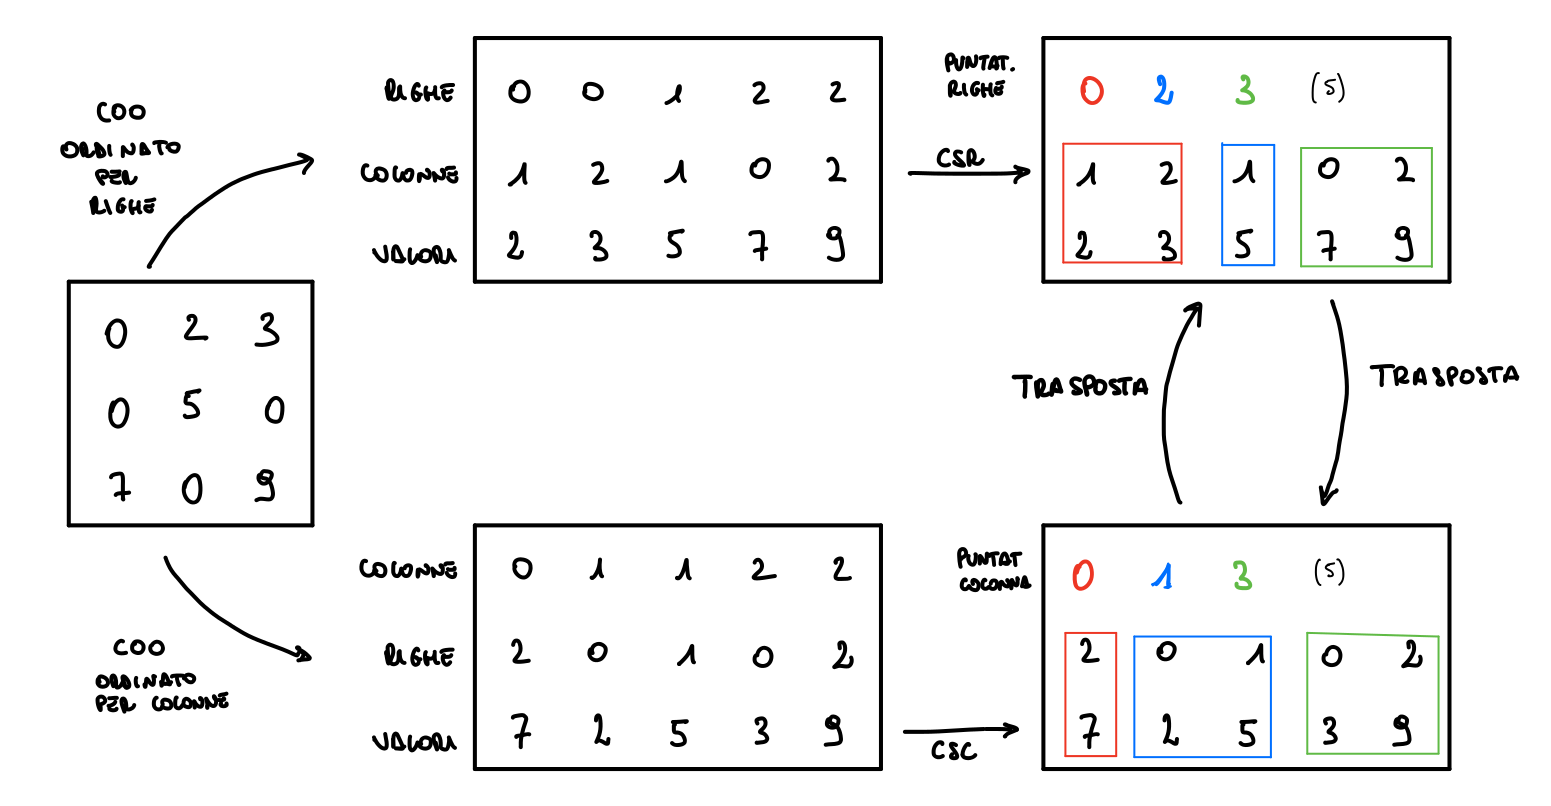
\includegraphics[scale=0.25]{conceptual_transpose.png}
	\caption{Trasformazione da formato esteso a CSR, oppure CSC}
	\label{first_fig}
\end{figure*}

\section{Introduzione e motivazioni}\label{introduzione}

	% problema e motivazioni
	Sempre più applicazioni computazionali in ambito scientifico necessitano di algoritmi che compiano operazioni applicabili su matrici sparse. Si parla di semplici operazioni di algebra lineare, di moltiplicazione o di calcolo della trasposta come in questo caso.\newline
	Il problema analizzato, quello della trasposizione di matrici, si presta bene al calcolo parallelo per l'esecuzione in maniera più efficiente e veloce. Verranno quindi mostrate le basi per la rappresentazione, i problemi riscontrati durante lo sviluppo e analizzati alcuni algoritmi per il calcolo su \textit{Gpu}.\newline


\section{Rappresentazione delle matrici}
\label{rappresentazione}
	Una matrice sparsa non è altro che una matrice i cui valori sono per la maggior parte uguali a zero. La matrice in formato classico necessita di una quantità di memoria minima di $ m $x$ n $ elementi, ma essendo l'obiettivo quello di lavorare su matrici sparse non è stato necessario e utile memorizzare la matrice in formato denso.\newline
	Per rappresentare in modo efficace le matrici sparse senza troppo utilizzo di memoria sono state quindi introdotte ed utilizzate delle forme di rappresentazione matriciale che permettono il salvataggio di dati utilizzando quantitativi di memoria inferiori.\newline
	Di seguito vengono spiegate le due metodologie da noi utilizzate.
	
	\subsection{Formato Csr}
	\label{csr}
	Il \textit{compressed sparse row} è una rappresentazione di una matrice $ M $ basata su tre array monodimensionali, che rispettivamente contengono:
	\begin{enumerate}
		\item \textit{V}: i valori non zero (\textit{nnz}),
		\item \textit{COL\_INDEX}: gli indici delle colonne dove si trovano gli elementi \textit{nnz},
		\item \textit{ROW\_INDEX}: ha un elemento per ogni riga della matrice e rappresenta l'indice in $ V $ dove comincia la riga data.
	\end{enumerate}
	I primi due array sono di dimensione \textit{nnz}, mentre il terzo array è al massimo di dimensione $ m $.
	
	\subsection{Formato Csc}
	\label{csc}
 	Questa metodologia per la rappresentazione è simile alla precedente citata \textit{Csr}, a differenza che i valori vengono letti prima per colonna. Di conseguenza, un indice di riga viene memorizzato per ogni valore e lo stesso viene fatto per i puntatori di colonna .
 	
	\subsection{Da Csr a Csc}
	\label{csr-to-csc}
 	Per il problema della trasposta di matrice è stato quindi utile introdurre entrambe le rappresentazioni. Infatti, ogni algoritmo  descritto in sezione~\ref{metodologie}, necessita di sei array per effettuare il calcolo della trasposta e dare l'output nella tipologia corretta. Abbiamo quindi:
 	\begin{itemize}
 		\item in input il formato \textit{Csr}: csrRowPtr, csrColIdx, csrVal;
 		\item in output il formato \textit{Csc}: cscColPtr, cscRowIdx, cscVal.	
 	\end{itemize}
 	In base a come vengono create le matrici, se in modo casuale oppure se lette da file, vengono effettutate delle operazioni preliminari descritte dalla procedure in sezione~\ref{procedure} che portano ad ottenere gli array in input e in output nel formato corretto per effettuarne il controllo di correttezza.\newline

\section{Metodologie analizzate}
\label{metodologie}
	In questa sezione vengono spiegate ed evidenziate le differenze tra le varie metodologie analizzate. 
		
	\subsection{Trasposta seriale}
%	La prima metodologia descritta è quella seriale. Sempre a partire dalla rappresentazione in formato \textit{csr} della matrice iniziale l'algoritmo crea un array di elementi, dove per ogni colonna della matrice analizzata conta quanti elementi \textbf{nnz} ci sono. Possiamo definire questo array come un istogramma delle frequenze degli elementi delle colonne. 
	La prima metodologia descritta è quella seriale. Sempre a partire dalla rappresentazione in formato \textit{csr} della matrice iniziale l'algoritmo ottiene i puntatori alle colonne (formato csc) a partire dagli indici di colonna (formato csr). Viene quindi applicato un algoritmo seriale di \textit{prefix\_sum} su questo array, per ottenere i valori corretti di \textbf{cscColPtr}. Infine gli indici di riga e i valori nel nuovo formato \textit{csc} vengono sistemati.\newline
	Questa implementazione servirà come base sulla quale verranno eseguiti i controlli degli algoritmi successivamente implementati.
	
	\subsection{Nvidia cuSPARSE}
	Questo toolkit è implementato all'interno nelle librerie NVIDIA CUDA runtime. Le routine delle librerie vengono utilizzate per operazioni tra vettori e matrici che sono rappresentate tramite diversi formati. Inoltre mette a disposione operazioni che permettono la conversione attraverso diverse rappresentazioni di matrici. Supporta inoltre la compressione in formato \textit{csr} che è una delle più usate quando si vuole rappresentare matrici sparse in modo efficiente.\newline	
	Il codice è stato sviluppato partendo dalla guida \cite{cusparse} ed è diviso in due versioni di cuSPARSE a causa delle Gpu utilizzate. In fase di compilazione viene quindi controllata la versione usata: $ 9 $ o $ 10 $.\newline
	Nel caso in cui la versione usata sia la $ 10 $ vengono svolti alcuni ulteriori passi, come l'allocazione dello spazio necessario per l'esecuzione di cuSparse oltre all'allocazione del buffer per il calcolo della trasposta. Per quanto riguarda la versione $ 9 $ invece questi passi non sono necessari.\newline
	Infine viene chiamata la procedura che effettua il calcolo della trasposta. Nel caso in cui la versione di cuSPARSE sia la $ 10 $ viene richiesto come ulteriore parametro l'algoritmo da utilizzare.\newline
	Dopo essere state eseguite entrambe ritornano i valori ottenuti in formato \textit{csc}.

	\subsection{ScanTrans}
	L'algoritmo considerato prevede di effettuare la trasposta di matrici basandosi sul concetto di scan. Partendo sempre dal presupposto di avere in input una matrice in formato \textit{Csr}, vengono costruiti due array ausiliari:
	\begin{itemize}
		\item inter: array bidimensionale di dimensione $ (nthreads+1) * n $,
		\item intra: array monodimensionale di dimensione massima $ nnz $.
	\end{itemize}
	Ogni riga in \textit{inter} contiene il numero di indici della colonna presi dalla thread i-esima. Mentre ogni elemento in \textit{intra} viene utilizzato per salvare l'offeset relativo alla colonna corrispondente all'elemento nnz preso dalla thread. Dopo aver ottenuto gli istogrammi, viene applicato un \textit{vertical scan} su inter, e una \textit{prefix sum} solamente sull'ultima riga di inter. Infine l'algoritmo calcola l'offset assoluto relativo ad ogni elemento nnz e ritorna il tutto in formato \textit{csc}.\newline
	Tutte le procedure utilizzate in \textit{Scan Trans} si trovano in sezione \ref{procedure}, e vengono eseguite nel seguente ordine:
	\begin{enumerate}
		\item pointers to index: \ref{pnt-to-idx},
		\item index to pointers: \ref{idx-to-pnt},
		\item scan: \ref{scan},
		\item reorder elements.
	\end{enumerate}
	
	\begin{figure}[H]
		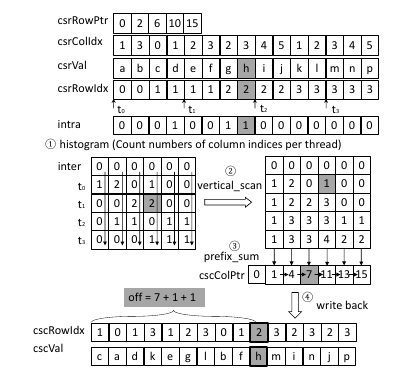
\includegraphics[scale=0.6]{scantrans.png}
		\caption{Scan Trans, esempio utilizzato in \cite{parallelTrans}.}
		\label{scantrans}
	\end{figure}
	
	\subsection{MergeTrans}
	L'algoritmo considerato prevede due passi importanti: \textit{sort} e \textit{merge}.
	Inizialmente sono stati creati gli indici di riga a partire dai puntatori delle colonne e su questi ultimi è stato fatto un sort su piccole porzioni di array, mantenendo quindi i vari blocchi disordinati tra di loro ma con gli elementi ordinati. Successivamente è stato utilizzato il merge ricorsivo partendo dai blocchi più piccoli e unendoli in blocchi sempre più grandi. Per funzionare questo processo necessita dell'utilizzo di due buffer di memoria che contengono gli elementi appena ordinati. Infine dai puntatori delle colonne vengono estraxtti gli indici e viene fatta la scan che ritorna il risultato in formato \textit{csc}. \newline
	Anche in questo caso le procedure utilizzate si trovano in sezione \ref{procedure}, e sono ordinatamente eseguite come segue:
	\begin{enumerate}
		\item pointers to index: \ref{pnt-to-idx},
		\item segmented sort: \ref{seg-sort},
		\item segmented merge: \ref{merge},
		\item index to pointers: \ref{idx-to-pnt},
		\item scan: \ref{scan}.
	\end{enumerate}
	
	\begin{figure}[H]
		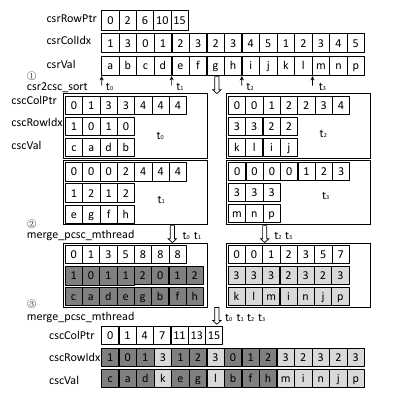
\includegraphics[scale=0.6]{mergetrans.png}
		\caption{Merge Trans, esempio utilizzato in \cite{parallelTrans}.}
		\label{mergetrans}
	\end{figure}
	
% Inserimento sezione delle procedure

\section{Procedure}\label{procedure}

I due algoritmi \ScanTrans e \MergeTrans vengono scomposti in diversi componenti, ognuno dei quali viene valutato nelle performance e testato separatamente. 

\subsection{Scan}
\label{scan}
Questa operazione prende in input un vettore $A = (a_0, a_1, ..., a_n)$ e ritorna un vettore $B=(I, a_0, a_0 \oplus a_1, ..., a_0 \oplus a_1 \cdots \oplus a_{n-1})$ con $\oplus$ è un'operazione binaria il cui elemento identità è $I$. Nel nostro caso l'operazione è la somma. 

L'algoritmo apparentemente sembra difficile da parallelizzare in quanto il risultato di ogni elemento dipende da tutti i gli elementi precedenti. Diverse soluzioni sono state proposte tra cui l'\emph{algoritmo di Blelloch}. Il suo funzionamento in due fasi è illustrato in Figura~\ref{scan_blelloch} e dettagliatamente discusso in \cite{scan}.

\begin{figure}[H]
	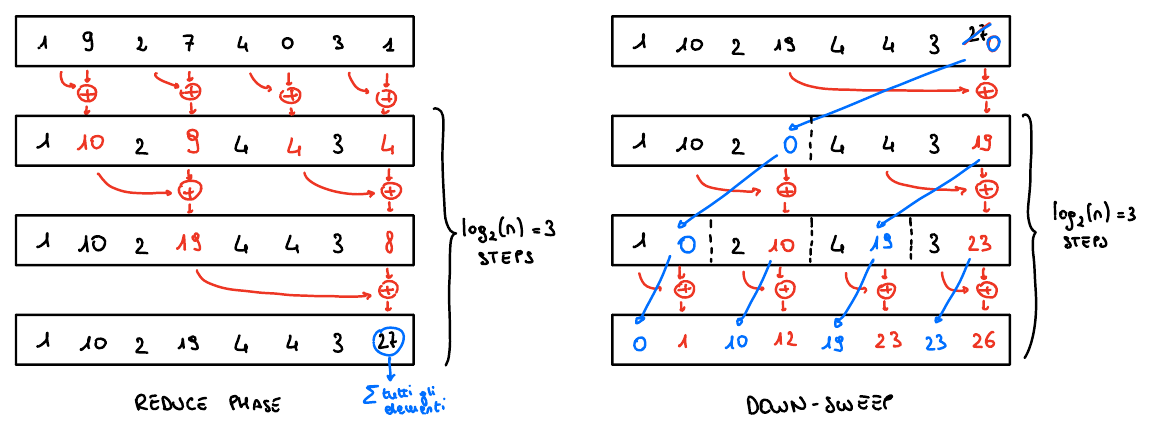
\includegraphics[scale=0.3]{scan.png}
	\caption{Algoritmo di Blelloch}
	\label{scan_blelloch}
\end{figure}

L'implementazione prevede che se l'intero vettore riesce ad essere memorizzato all'interno della shared memory di $N$ elementi, allora possiamo calcolare scan con una singola chiamata a kernel. 

Nel caso questo non sia possibile, l'operazione di scan viene segmentata, applicata separatamente a blocchi di $N$ elementi. Successivamente si mantiene un vettore di somme (vettore degli ultimi elementi del blocco), si applica ricorsivamente \emph{scan} su esso e si sommano gli offset ottenuti all'intero vettore di partenza. 

\subsection{Segmented sort}
\label{seg-sort}
Questa operazione prende in input un vettore di lunghezza $n$ ed un intero $\BlockSize$. Il vettore viene diviso in segmenti di lunghezza $\BlockSize$. Gli elementi di ogni segmento vengono permutati in modo che siano ordinati stabilmente. L'intero segmento deve rientrare nella shared memory.  

\begin{figure}[H]
\centering
	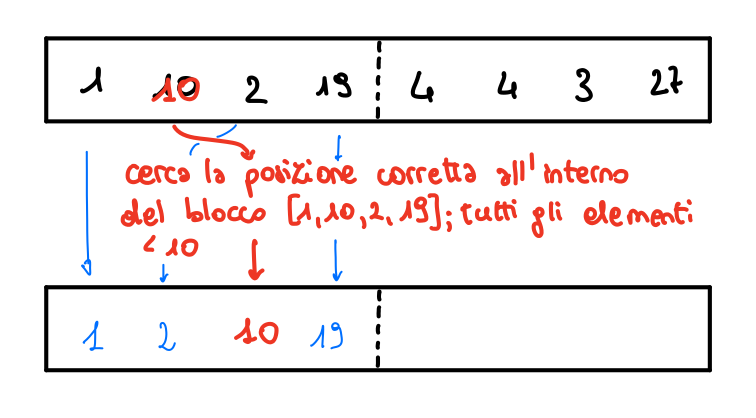
\includegraphics[scale=0.15]{segmented_sort.png}
	\caption{Segmented Sort}
	\label{segmented_sort}
\end{figure}

Una volta caricato il blocco in shared memory, la $i$-esima thread del blocco è incaricata di trovare la posizione corretta dell'$i$-esimo elemento all'interno del segmento, ed assegnarlo a tale posizione. L'algoritmo viene illustrato in Figura~\ref{segmented_sort}. 

L'ordinamento deve essere stabile quindi la posizione dell'$i$-esimo elemento di valore $y$ è dato dal numero di elementi $<y$, sommati al numero degli elementi $=y$ per indici $<i$. 

La dimensione ideale del blocco pari a $128$ elementi (caso interi a 32bit), ed è stata trovata empiricamente:
\begin{figure}[H]
	\centering
	\begin{tabular}{SS}
		\toprule
		\textbf{Thread per blocco} & \textbf{Performance (\si{\milli\second})} \\ \midrule
		128  & 2135.58 \\
		256  & 2139.62 \\
		512  & 2156.61  \\ \bottomrule
	\end{tabular}
	\caption{Performance su array di $2\cdot 10^7$ elementi}
\end{figure}

\subsection{Merge}
\label{merge}
L'operazione di \emph{merge} trasforma un vettore diviso in segmenti di dimensione $\BlockSize$ nel quale gli elementi di ogni segmento sono ordinati, in un vettore diviso in segmenti ordinati di dimensione $2 * \BlockSize$, ognuno dei quali è l'unione di una coppia di blocchi contigui. 

Differenziamo il caso in cui il blocco di dimensione $\BlockSize$ rientri o meno nella shared memory. 

\subsection{Merge small}

In questo caso una coppia di blocchi rientra completamente nella shared memory. In modo analogo a quanto fatto per l'operazione di \emph{segmented sort}, abbiamo un numero di thread per blocco pari a $\BlockSize$ nel quale l'$i$-esimo thread è incaricato di calcolare la posizione dell'$i$-esimo elemento. 

In questo caso la posizione dell'$i$-esimo elemento del blocco di sinistra è $i+j$ con $j$ posizione dell'elemento all'interno del blocco di destra, trovato attraverso una ricerca binaria in quanto i blocchi sono ordinati (differentemente da quanto avviene per il segmented sort). Analogamente lo stesso avviene per gli elementi del blocco di destra. 

A parità di valore, gli elementi del blocco di sinistra hanno indice minore di quelli di destra. 

\subsection{Merge big}

\begin{figure}[t]
    \centering
	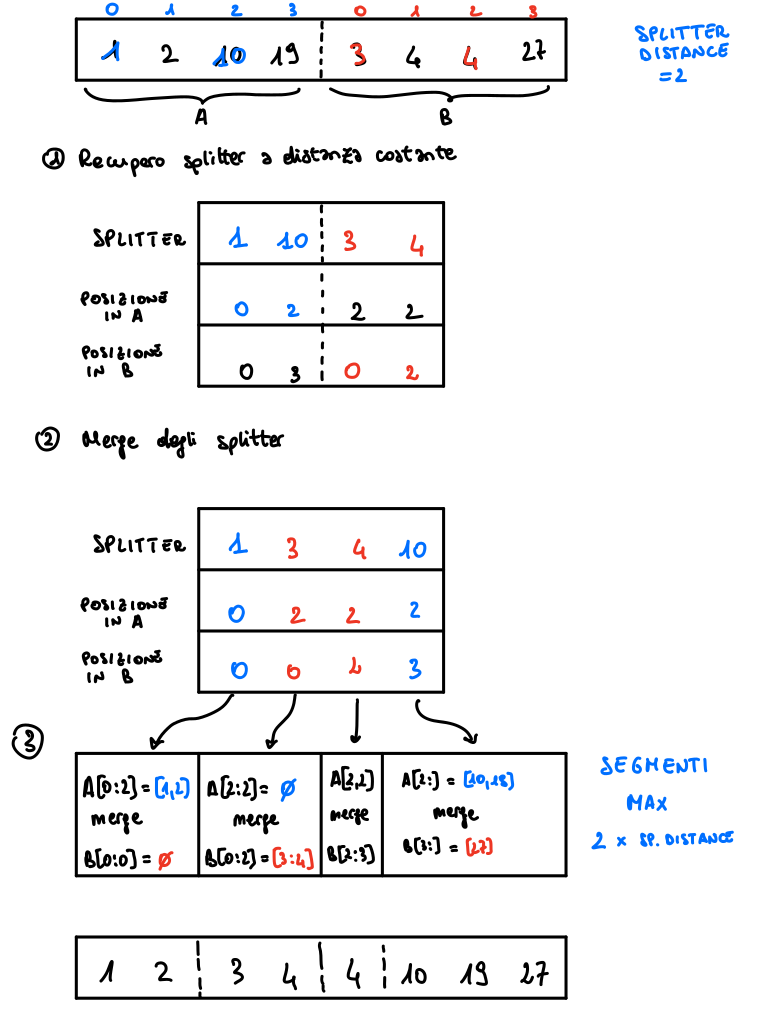
\includegraphics[scale=0.3]{merge_big.png}
	\caption{Merge big}
	\label{merge_big}
\end{figure}

Questo secondo algoritmo è illustrato in Figura~\ref{merge_big} ed originariamente preso da \cite{mergebig}. Applicando sempre \emph{merge small}, oltre che rinunciare alla shared memory, ogni thread del blocco dovrebbe lavorare su più di un elemento, aumentando la complessità della procedura. 

L'algoritmo proposto funziona nel seguente modo:
\begin{enumerate}
    \item recuperiamo dal vettore degli elementi segnaposto detti \emph{splitter} presi a distanza costante e pari ad $\SplitterDistance$; \\
    per ogni coppia di segmenti da unire ho una coppia di blocchi di splitter, trovo quindi la posizione di ogni splitter all'interno del blocco di destra ($A$) e di sinistra ($B$);
    \item applico \emph{merge} ricorsivamente sugli array di splitter;
    \item gli indici associati agli splitter dividono la coppia di blocchi in modo tale da poter effettuare tanti merge indipendenti da quanti sono gli splitter. \emph{Ogni merge indipendente considererà al massimo $2* \SplitterDistance$ elementi} (numero costante che scegliamo tale che rientri nella shared memory).
\end{enumerate}

La dimensione ideale del blocco pari a $256$ elementi (caso interi a 32bit), ed è stata trovata empiricamente:
\begin{figure}[H]
	\centering
	\begin{tabular}{SS}
		\toprule
		\textbf{Thread per blocco} & \textbf{Performance (\si{\milli\second})} \\ \midrule
		128  & 708.87  \\	
		256  & 701.54 \\
		512  & 715.71 \\ \bottomrule
	\end{tabular}
	\caption{Performance su array di $2\cdot 10^7$ elementi}
\end{figure}
Mentre il valore migliore per la distanza degli splitter (\SplitterDistance) è di $ 128 $.

\subsection{Istogramma / Index to pointers}
\label{idx-to-pnt}
Dato un vettore $A$ di $n$ elementi compresi tra $0$ ed $m-1$ riceviamo un vettore di $m$ elementi nel quale l'$i$-esima cella contiene la frequenza con cui il valore $i$ è presente in $A$. 

L'algoritmo si sviluppa in due fasi:
\begin{enumerate}
    \item il vettore $A$ viene diviso in $N$ segmenti di lunghezza omogenea, ogni segmento viene processato da un blocco di thread che mantiene l'istogramma parziale;
    \item gli istogrammi parziali vengono poi uniti attraverso un'operazione di prefix scan che si effettua ``in verticale''. Tale operazione può essere ottenuta:
    \begin{itemize}
        \item trasponendo la matrice degli istogrammi parziali ed applicando $N$ volte \emph{prefix sum}; oppure
        \item attraverso $N$ blocchi di thread che attraversano sequenzialmente il vettore colonna degli istogrammi parziali.
    \end{itemize}
    \item si applica \emph{prefix sum} sul risultato dell'operazione precedente.
\end{enumerate}

L'algoritmo è illustrato in Figura~\ref{index_to_pointers}. 

\begin{figure}[t]
    \centering
	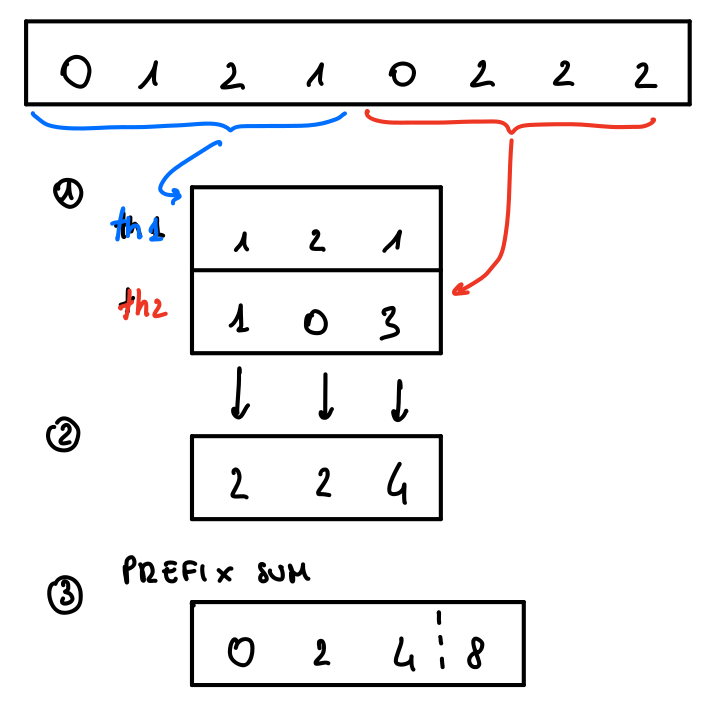
\includegraphics[scale=0.22]{index_to_pointers.png}
	\caption{Index to pointers}
	\label{index_to_pointers}
\end{figure}


La dimensione ideale del blocco pari a $32$ elementi (caso interi a 32bit), ed è stata trovata empiricamente:
\begin{figure}[H]
	\centering
	\begin{tabular}{SS}
		\toprule
		\textbf{Thread per blocco} & \textbf{Performance (\si{\milli\second})} \\ \midrule
		1 & 1016.87 \\
		32 & 1013.65 \\
		64 & 1024.70 \\
		256 & 986.84 \\ \bottomrule
	\end{tabular}
	\caption{Performance su array di $10^6$ elementi} % da 999'999 a 1'000'000
\end{figure}

\subsection{Pointers to index}
\label{pnt-to-idx}
Operazione inversa di \emph{index to pointers}. Il vettore risultante è ordinato. Può essere implementato assegnando ad ogni blocco di thread un elemento del vettore delle frequenze da espandere. 

L'algoritmo è illustrato in Figura~\ref{pointers_to_index}. 

\begin{figure}[t]
    \centering
	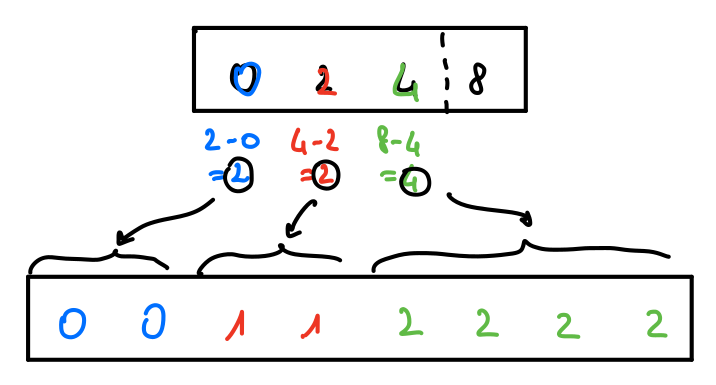
\includegraphics[scale=0.22]{pointers_to_index.png}
	\caption{Pointers to index}
	\label{pointers_to_index}
\end{figure}

La dimensione ideale del blocco pari a $32$ elementi (caso interi a 32bit), ed è stata trovata empiricamente:
\begin{figure}[H]
	\centering
	\begin{tabular}{SS}
		\toprule
		\textbf{Thread per blocco} & \textbf{Performance (\si{\milli\second})} \\ \midrule
		1 & 2328.88 \\
		16 & 2375.74 \\
		32 & 2322.75 \\
		1024 & 3326.13 \\ \bottomrule
	\end{tabular}
	\caption{Performance su array di $2\cdot 10^7$ elementi} 
\end{figure}



\section{Struttura dell'implementazione}\label{struttura}

L'intera implementazione è scaricabile attraverso \emph{git} dalla repository \url{https://github.com/michelepenzo/architetture-avanzate}.

La struttura delle directory del progetto è presente in Figura~\ref{fig:struct}. 

La sottodirectory \emph{doc} contiene questo stesso documento in formato \emph{pdf} ed i rispettivi sorgenti \emph{tex}. 

La sottodirectory \emph{code} contiene i sorgenti dell'applicativo principale e di quello secondario di test. 

Lo scopo del primo è generare un file \emph{csv} contente le tempistiche e gli speedup di ogni algoritmo applicato sulle istanze di matrici in input generate casualmente oppure lette da file \emph{mtx} (\emph{market matrix}, una rappresentazione della matrice sparsa in formato COO attraverso file di testo). 

Lo scopo del secondo applicativo è testare il corretto funzionamento di ogni componente del progetto. In particolare, vengono sottoposte le stesse istanze di array o matrici (a seconda del componente che sta per essere testato) sia alla funzione che ne implementa l'algoritmo parallelo, sia alla funzione che ne implementa l'algoritmo seriale. Ovviamente ci si aspetta che i risultati siano uguali per tutte le istanze.

\begin{figure}
    \dirtree{%
	.1 root.		
	    .2 README.md.
		.2 doc.			
		.2 code.
			.3 {matrices}.
			.3 {include}.
				.4 {matrix.hh}.
				.4 {merge\_step.hh}.
				.4 {procedures.hh}.
				.4 {transposers.hh}.
				.4 {Timer.$ * $}.
				.4 {utilities.hh}.
			.3 {src}.
				.4 {...}.
				.4 {transposer.cu}.
				.4 {main.cu}.
			.3 {test}.	
				.4 {...}.
				.4 {tester.hh}.
				.4 {test\_main.cu}.
			.3 Makefile.			
			.3 {timing\_analysis.csv}.	
}
    \caption{Struttura delle directory del progetto}
    \label{fig:struct}
\end{figure}

In particolare:
\begin{itemize}
    \item il file \texttt{include/matrix.hh} contiene le classi \emph{FullMatrix} e \emph{SparseMatrix} che si occupano di allocare nella memoria host lo spazio necessario a contenere la matrice date le sue specifiche ($m$, $n$, $nnz$), sia come matrice estesa sia in formato \emph{csr}. Inoltre contiene i metodi per inizializzare la matrice in modo casuale e per passare da un formato all'altro;
    \item il file \texttt{include/utils.hh} contiene i metodi di utilità quali le funzioni di stampa e di allocazione e deallocazione della memoria device;
    \item i file \texttt{include/procedures.hh} e \texttt{merge\_step.hh} contengono le dichiarazioni delle procedure descritte nella Sezione~\ref{procedure}. La maggior parte delle definizioni sono presenti nella sottodirectory \texttt{src}, nel caso del metodo \emph{merge\_step} la definizione è scritta direttamente nell'header. Questa scelta è conveniente in quanto tale funzione è definita rispetto ad un tipo generico, se la definizione fosse stata riportata nei file cpp avremmo dovuto indicare esplicitamente i tipi concreti per il quale vogliamo rendere disponibile il nostro metodo (\cite{template});
    \item il file \texttt{include/transposers.hh} e rispettivo sorgente \texttt{src/transposers.cu} contengono le dichiarazioni e definizioni dei metodi che effettuano la trasposta: seriale, parallela con \ScanTrans{} e \MergeTrans{} ed infine da libreria \cuSPARSE{} con entrambi i possibili algoritmi;
    \item i file \texttt{Timer.*} contengono una classe di utilità \emph{timer} che permette di cronometrare il tempo che occorre per eseguire un dato pezzo di codice;
    \item il file \texttt{src/main.cu} contiene l'applicativo principale che chiama i diversi metodi di trasposta sulla matrice fornita in input, ne cronometra le tempistiche e le stampa in output;
    \item il file \texttt{test/tester.hh} contiene la classe astratta \emph{tester} che espone un metodo \emph{test\_many\_instances} che chiama un metodo astratto \emph{test} un numero arbitrario di volte, passandogli in input un intero che rappresenta il numero dell'istanza attuale che può essere usato per decidere la dimensione dell'istanza di test. Attualmente le istanze testate vanno da 1 a 20'000, poi da 20'000 a 20'000'000 con step $\times 1.5$; 
    \item i file \texttt{test/tester\_*.hh} si occupano di testare un singolo componente, contengono ciascuna uno o più classi concrete che estendono la classe astratta \emph{tester};
    \item il file \texttt{test/test\_main.cu} contiene l'applicativo di test che alloca oggetti delle varie classi tester, li avvia e ne stampa gli eventuali errori a video.
\end{itemize}
	
\section{Avvio degli applicativi}

L'applicativo principale può essere avviato con tre modalità diverse:
\begin{itemize}
    \item senza parametri, genera una matrice $500'000\times 500'000$ con $10'000'000$ elementi non nulli, ne valuta le tempistiche con i diversi algoritmi ritornando la media su un numero arbitrario di esecuzioni;
    \item con tre parametri interi $\mathrm{m}$, $\mathrm{n}$, $\mathrm{nnz}$, genera una matrice avente le dimensioni ricevute in input e procede alla valutazione delle tempistiche come sopra;
    \item con un parametro stringa \texttt{filename}, legge da file una matrice che deve essere nel formato \emph{mtx market matrix}.
\end{itemize}

Avviando l'applicativo principale attraverso il Makefile con \emph{make run} viene avviato molteplici volte l'applicativo principale, ogni volta con un'istanza di matrice diversa in input, con lo scopo di popolare un documento \emph{timing\_analysis.csv} contenente le tempistiche medie su diversi input. 

L'applicativo di test di avvia con una sola modalità equivalentemente avviando il nome dell'applicativo senza parametro oppure attraverso il Makefile con \emph{make test}. Su \emph{stdout} viene stampato ``no" se almeno un test ha mostrato anomalie, ``ok" altrimenti. 


\begin{figure*}[t]
    \centering
    \scalebox{0.9}{
    \begin{tabular}{lS[table-format=7.0] S[table-format=7.0] S[table-format=8.0] S[table-format=4.2] S[table-format=4.2] S[table-format=4.2] S[table-format=4.2] S[table-format=4.2]}
    \toprule
    \textbf{Nome} 
    & \textbf{M}
    & \textbf{N}
    & \textbf{NNZ}
    & \textbf{Serial}
    & \textbf{\ScanTrans{}}
    & \textbf{\MergeTrans{}}
    & \textbf{\cuSPARSE{} 1}
    & \textbf{\cuSPARSE{} 2}
    \\ \midrule
    language.mtx	
        & 399130
        & 399130
        & 1216334
        &  55.75
        & 114.71
        & 197.05
        & 122.02
        &  18.36 \\
    webbase-1M.mtx	
        & 1000005	
        & 1000005
        & 3105536	
        & 138,84	
        & 278,55	
        & 520,90
        & 149,81	
        &  51,00 \\
    rajat21.mtx	
        & 411676	
        & 411676	
        & 1893370	
        &  77,97	
        & 147,64	
        & 306,56	
        & 127,31	
        &  26,77 \\
    ASIC\_680k.mtx	
        & 682862	
        & 682862	
        & 3871773	
        & 154,37	
        & 265,47	
        & 844,76	
        & 155,31	
        &  56,74 \\
    memchip.mtx	
        & 2707524	
        & 2707524	
        & 14810202	
        &  594,18	
        &  994,62	
        & 2328,67	
        &  298,93	
        &  188,07 \\
    cant.mtx	
        & 62451	
        & 62451	
        & 2034917	
        &  73,83	
        & 114,40	
        & 248,49	
        & 127,26	
        &  31,11 \\
    FullChip.mtx	
        & 2987012	
        & 2987012	
        & 26621990	
        &  997,37	
        & 1543,02	
        & 9481,42	
        &  454,53	
        &  328,32 \\
    stomach.mtx	
        & 213360	
        & 213360	
        & 3021648	
        & 110,84	
        & 164,30
        & 387,78	
        & 139,57	
        &  40,26 \\
    web-Google.mtx	
        & 916428	
        & 916428	
        & 5105039	
        &  399,63	
        &  382,37	
        & 3327,56	
        &  170,59	
        &   73,25 \\
    random	
        & 100000	
        & 100000	
        & 10000000	
        &  898,99	
        &  475,17	
        & 3056,12	
        &  210,57	
        &  130,25 \\
    random	
        & 100000	
        & 100000	
        & 10000000	
        &  902,23	
        &  475,72	
        & 3060,25	
        &  208,22	
        &  133,22 \\
    random	
        & 150000	
        & 200000	
        & 5000000	
        &  523,66	
        &  263,90	
        & 1351,83	
        &  161,90	
        &   72,70 \\
    random	
        & 150000	
        & 200000	
        & 5000000	
        &  527,15	
        &  262,88	
        & 1353,93	
        &  165,19	
        &   74,98 \\
    random	
        & 500000	
        & 500000	
        & 10000000	
        & 1380,96	
        &  532,76	
        & 2853,55	
        &  227,33	
        &  141,18 \\ \bottomrule
    \end{tabular}}
    \caption{Risultati sperimentali -  $\textrm{M}, \textrm{N}, \textrm{NNZ}$ rispettivamente numero di righe, di colonne, di elementi non nulli della matrice. I tempi sono in \si{\milli\second}.}
    \label{results}
\end{figure*}

\begin{figure*}[t]
    \centering
    \scalebox{0.9}{
    \begin{tabular}{lS[table-format=7.0] S[table-format=7.0] S[table-format=8.0] S[table-format=4.2] S[table-format=4.2] S[table-format=4.2] S[table-format=4.2] S[table-format=4.2]}
    \toprule
    \textbf{Nome} 
    & \textbf{M}
    & \textbf{N}
    & \textbf{NNZ}
    & \textbf{Serial}
    & \textbf{\ScanTrans{}}
    & \textbf{\MergeTrans{}}
    & \textbf{\cuSPARSE{} 1}
    & \textbf{\cuSPARSE{} 2}
    \\ \midrule
    language.mtx	
        & 399130	
        & 399130	
        & 1216334	
        & 1.00
        & 0.49	
        & 0.28	
        & 0.46	
        & 3.04 \\
    webbase-1M.mtx	
        & 1000005	
        & 1000005	
        & 3105536	
        & 1.00
        & 0.50	
        & 0.27	
        & 0.93	
        & 2.72 \\
    rajat21.mtx	
        & 411676	
        & 411676	
        & 1893370	
        & 1.00
        & 0.53	
        & 0.25	
        & 0.61	
        & 2.91 \\
    ASIC\_680k.mtx	
        & 682862	
        & 682862	
        & 3871773	
        & 1.00
        & 0.58	
        & 0.18	
        & 0.99	
        & 2.72 \\
    memchip.mtx	
        & 2707524	
        & 2707524	
        & 14810202	
        & 1.00
        & 0.60	
        & 0.26	
        & 1.99	
        & 3.16 \\
    cant.mtx	
        & 62451	
        & 62451	
        & 2034917	
        & 1.00
        & 0.65	
        & 0.30	
        & 0.58	
        & 2.37 \\
    FullChip.mtx	
        & 2987012	
        & 2987012	
        & 26621990	
        & 1.00
        & 0.65	
        & 0.11	
        & 2.19	
        & 3.04 \\
    stomach.mtx	
        & 213360	
        & 213360	
        & 3021648	
        & 1.00	
        & 0.67	
        & 0.29	
        & 0.79	
        & 2.75 \\
    web-Google.mtx	
        & 916428	
        & 916428	
        & 5105039	
        & 1.00
        & 1.05	
        & 0.12	
        & 2.34	
        & 5.46 \\
    random	
        & 100000	
        & 100000	
        & 10000000	
        & 1.00	
        & 1.89	
        & 0.29	
        & 4.27	
        & 6.90 \\
    random	
        & 100000	
        & 100000	
        & 10000000	
        & 1.00	
        & 1.90	
        & 0.29	
        & 4.33	
        & 6.77 \\
    random
        & 150000	
        & 200000	
        & 5000000	
        & 1.00	
        & 1.98	
        & 0.39	
        & 3.23	
        & 7.20 \\
    random
        & 150000	
        & 200000	
        & 5000000	
        & 1.00	
        & 2.01	
        & 0.39	
        & 3.19	
        & 7.03 \\
    random
        & 500000	
        & 500000	
        & 10000000	
        & 1.00	
        & 2.59	
        & 0.48	
        & 6.07	
        & 9.78 \\ \bottomrule
    \end{tabular}}
    \caption{Risultati sperimentali -  Speedup}
    \label{results_speedup}
\end{figure*}






\section{Risultati sperimentali}

Confrontiamo ora le performance delle varie implementazioni che seguono:
\begin{itemize}
    \item seriale;
    \item parallela \emph{scan trans};
    \item parallela \emph{merge trans};
    \item \cuSPARSE (entrambi gli algoritmi).
\end{itemize}

Le istanze su cui vengono eseguiti i vari algoritmi sono in parte generate in modo casuale (a partire dalle specifiche della matrice sparsa), in parte recuperate dal dataset "University  of Florida sparse  matrix collection`` \cite{dataset}. Tale dataset è stato usato per valutare le performance degli algoritmi in \cite{parallelTrans}.

La macchina sul quale vengono eseguiti i vari algoritmi è equipaggiata con una scheda NVidia GeForce GTX 780 con Cuda Runtime 10.2.

I risultati sono visibili in Tabella~\ref{results}. 

\section{Considerazioni finali}\label{conclusioni}
	% tirare le somme di cosa abbiamo ottenuto
	% cosa migliorare?
	% come possiamo continuare il progetto se avessimo avuto più tempo?
		% algo merge con merge buffer che è gia implementato
		% testare l'efficienza delle componenti rispetto alla implementazione nvidia
		% idx to pntrs (soffre race condition) --> un thread ha un blocco
		
% TODO
\newpage
\bibliographystyle{IEEEtran}
\bibliography{biblio}


%\appendix
%Se non avete abbastanza spazio, potete inserire le figure delle EFSM in una  pagina extra, appendice. Un esempio di come potete fare solo le Figure~\ref{fig:grande}, \ref{fig:piccola1}, \ref{fig:piccola2}.

\end{document}